Based on the \textbf{acf} and \textbf{pacf} in (f), fit an appropriate seasonal ARIMA model to the log transformed Airlines Pasengers series. Make sure to explain why you select that model (model diagnostics).

\nl For the nonseasonal component, both the ACF and PACF cut off after lag 1. This would indicate either $\AR(1), \MA(1),$ or $\ARMA(1,1)$ to be a good starting model. 

\nl For the seasonal component, the ACF and PACF both appear to cut off after lag 1, though its not a perfectly clear seasonal drop, which would also be $\SAR(1), \SMA(1),$ or $\SARMA(1,1)$.

\nl When trying a $\SARIMA(1,1,1) \times (1,1,1)_{12}$ in R, we can look at the coefficents' p-values.
$$\texttt{sarima(stableAirpass, 1,1,1, 1,1,1, 12,no.constant=TRUE)}$$
\notab{\center{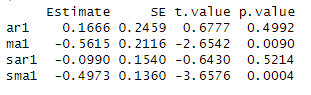
\includegraphics[width=3in]{img/7g.PNG}}}

\nl Dropping the ar1 and sar1 terms due to their large p-values yields a new model
$$\texttt{sarima(stableAirpass, 0,1,1, 0,1,1, 12,no.constant=TRUE)}$$
\notab{\center{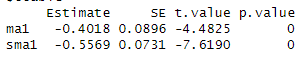
\includegraphics[width=3in]{img/7g2.PNG}}}
With the following diagnostic plots:

\notab{\center{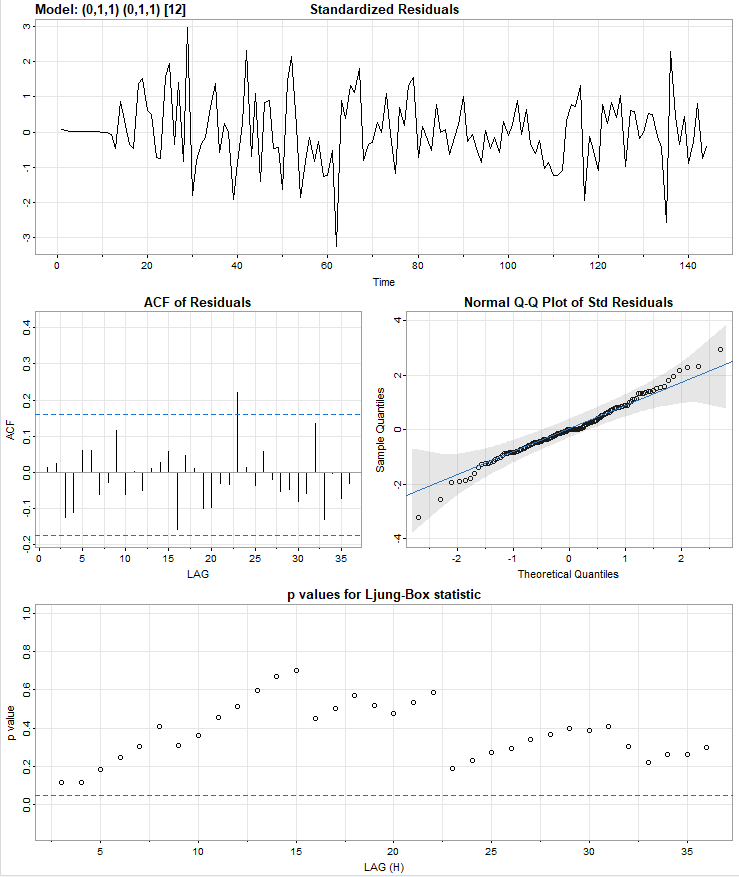
\includegraphics[width=6in]{img/7gPlots.PNG}}}

The Ljung-Box statistic being greater than $\alpha = 0.05$ indicates iid residuals and the QQ plot indicates normally distributed residuals. The R console results also show an estimated $\sigma^2 = 0.0013$ which is very low, along with an AIC of $-483.4$. This seems to be a very good model based on these additional numbers.